\chapter{Làm việc với dữ liệu trong n8n}

\section{Biến, JSON, Expressions}

\subsection{Biến trong n8n: Cách lưu trữ và sử dụng thông tin}

Trong cuộc sống hàng ngày, chúng ta thường ghi chú thông tin để sử dụng sau này. Trong n8n, ``biến'' chính là những ghi chú kỹ thuật số.

\subsubsection{Ví dụ: Tự động gửi tin nhắn chào mừng}

Giả sử bạn muốn chào mừng khách hàng mới đăng ký:

\begin{enumerate}
    \item Tạo biến workflow để lưu lời chào:
    \begin{verbatim}
    welcomeMessage: Chào mừng bạn đến với dịch vụ của chúng tôi!
    companyName: Công ty ABC
    \end{verbatim}

    \item Khi có người đăng ký, sử dụng biến trong email:
    \begin{verbatim}
    Tiêu đề: {{ $vars.welcomeMessage }}
    Nội dung: Cảm ơn bạn đã đăng ký dịch vụ của {{ $vars.companyName }}
    \end{verbatim}
\end{enumerate}

% \begin{figure}[h]
%     \centering
%     \includegraphics[width=0.8\textwidth]{images/bien-trong-workflow-email}
%     \caption{Biến trong workflow thực tế}
%     \label{fig:bien-workflow}
% \end{figure}

\textbf{Cách thiết lập biến đơn giản:}
\begin{enumerate}
    \item Mở workflow
    \item Nhấp vào biểu tượng bánh răng
    \item Chọn ``Variables''
    \item Thêm tên và giá trị cho biến
\end{enumerate}

\subsection{JSON: Ngôn ngữ dữ liệu của n8n}

JSON giống như một bảng thông tin có tổ chức. Ví dụ, thông tin người dùng trong JSON:

\begin{verbatim}
{
  "hoTen": "Nguyễn Văn A",
  "email": "nguyenvana@example.com",
  "soDienThoai": "0912345678",
  "diaChi": {
    "duong": "Lê Lợi",
    "quan": "Hoàn Kiếm",
    "thanhPho": "Hà Nội"
  }
}
\end{verbatim}

\subsubsection{Thu thập thông tin biểu mẫu từ website}

Khi khách hàng điền form trên website:
\begin{enumerate}
    \item Thông tin được gửi đến n8n dưới dạng JSON
    \item Mỗi mục thông tin là một cặp key-value
    \item Dữ liệu có thể lồng nhau (như địa chỉ ở trên)
\end{enumerate}

\subsection{Expressions: Công cụ làm việc với dữ liệu}

(bổ sung cho phần trên)

Expressions giống như công thức trong Excel, giúp bạn tính toán và xử lý dữ liệu.

\subsubsection{Ví dụ: Tính giá sau giảm giá}

Giả sử bạn có shop online và muốn tính giá sau khi giảm 10\%:

\begin{enumerate}
    \item Trong Set node, tạo trường ``giaSauGiamGia'':
    \begin{verbatim}
    {{ $json.giaBanDau * 0.9 }}
    \end{verbatim}

    \item Định dạng giá tiền:
    \begin{verbatim}
    {{ ($json.giaSauGiamGia).toFixed(0).toString()
    .replace(/\B(?=(\d{3})+(?!\d))/g, ".") }}
    \end{verbatim}
\end{enumerate}

% \begin{figure}[h]
%     \centering
%     \includegraphics[width=0.8\textwidth]{images/expressions-tinh-gia}
%     \caption{Expressions tính giá giảm 10\%}
%     \label{fig:expressions-gia}
% \end{figure}

\textbf{Ứng dụng thực tế khác:}
\begin{enumerate}
    \item Chuyển đổi định dạng ngày: \verb|{{ new Date($json.ngayDatHang).toLocaleDateString('vi-VN') }}|
    \item Ghép họ và tên: \verb|{{ $json.ho + ' ' + $json.ten }}|
    \item Kiểm tra điều kiện: \verb|{{ $json.tuoi >= 18 ? 'Người lớn' : 'Trẻ em' }}|
\end{enumerate}

\section{Storage Node (Data, Cache, Database)}

\subsection{Data Storage: Lưu trữ thông tin giữa các lần chạy}

\subsubsection{Ví dụ: Đếm số lượt truy cập website}

\begin{enumerate}
    \item Mỗi khi có người truy cập:
    \begin{itemize}
        \item Lấy số lượt hiện tại từ Data Storage
        \item Tăng thêm 1
        \item Lưu lại vào Data Storage
    \end{itemize}
\end{enumerate}

% \begin{figure}[h]
%     \centering
%     \includegraphics[width=0.8\textwidth]{images/workflow-dem-luot-truy-cap}
%     \caption{Workflow đếm lượt truy cập website}
%     \label{fig:dem-luot-truy-cap}
% \end{figure}

\textbf{Các bước thực hiện:}
\begin{enumerate}
    \item Thêm HTTP Trigger (kích hoạt khi có truy cập)
    \item Thêm Data Storage node đầu tiên:
    \begin{itemize}
        \item Operation: Get
        \item Key name: visitCount
    \end{itemize}
    \item Thêm Function node để tăng số:
    \begin{verbatim}
    // Nếu chưa có dữ liệu, bắt đầu từ 0
    const currentCount = items[0].json.data ?
    parseInt(items[0].json.data) : 0;
    
    // Tăng thêm 1
    return [{ json: { count: currentCount + 1 } }];
    \end{verbatim}
    \item Thêm Data Storage node thứ hai:
    \begin{itemize}
        \item Operation: Set
        \item Key name: visitCount
        \item Value: \verb|{{ $json.count }}|
    \end{itemize}
\end{enumerate}

\subsection{Cache Node: Lưu trữ tạm thời}

\subsubsection{Ví dụ: Lưu cache kết quả tỷ giá tiền tệ}

Thay vì gọi API tỷ giá mỗi phút, bạn có thể:
\begin{enumerate}
    \item Gọi API tỷ giá
    \item Lưu kết quả vào Cache với thời hạn 1 giờ
    \item Các request trong 1 giờ tiếp theo sẽ dùng dữ liệu cache
\end{enumerate}

% \begin{figure}[h]
%     \centering
%     \includegraphics[width=0.8\textwidth]{images/workflow-cache-ty-gia}
%     \caption{Workflow cache tỷ giá tiền tệ}
%     \label{fig:cache-ty-gia}
% \end{figure}

\textbf{Thiết lập workflow:}
\begin{enumerate}
    \item Thêm Schedule Trigger (chạy mỗi phút)
    \item Thêm Cache node:
    \begin{itemize}
        \item Operation: Get
        \item Key name: exchangeRates
    \end{itemize}
    \item Thêm node IF (kiểm tra cache có dữ liệu không)
    \item Nếu không có dữ liệu:
    \begin{itemize}
        \item Gọi API tỷ giá qua HTTP Request
        \item Lưu kết quả vào Cache:
        \begin{itemize}
            \item Operation: Set
            \item Key name: exchangeRates
            \item TTL: 3600 (1 giờ)
        \end{itemize}
    \end{itemize}
\end{enumerate}

\subsection{Database Node: Làm việc với cơ sở dữ liệu}

\subsubsection{Ví dụ: Hệ thống đặt hàng đơn giản}

\begin{enumerate}
    \item \textbf{Lưu đơn hàng mới:}
    \begin{itemize}
        \item Khách điền form $\rightarrow$ HTTP Trigger nhận dữ liệu
        \item Lưu thông tin vào database:
        \begin{itemize}
            \item Operation: Insert
            \item Table: donhang
            \item Columns \& Values: thông tin từ form
        \end{itemize}
    \end{itemize}
\end{enumerate}


\begin{enumerate}\setcounter{enumi}{1}
    \item \textbf{Cập nhật trạng thái đơn hàng:}
    \begin{itemize}
        \item Admin cập nhật $\rightarrow$ HTTP Trigger
        \item Cập nhật database:
        \begin{itemize}
            \item Operation: Update
            \item Table: donhang
            \item Set: \verb|{{ $json }}|
            \item Where: id = \verb|{{ $json.id }}|
        \end{itemize}
    \end{itemize}

    \item \textbf{Tạo báo cáo đơn hàng theo ngày:}
    \begin{itemize}
        \item Trigger chạy vào cuối ngày
        \item Truy vấn database:
        \begin{itemize}
            \item Operation: Select
            \item Table: donhang
            \item Where: ngayDatHang = today
        \end{itemize}
        \item Gửi email báo cáo tới quản lý
    \end{itemize}
\end{enumerate}

\section{HTTP Request \& API Basics}

\subsection{Tương tác với API: Lấy thông tin từ dịch vụ bên ngoài}

\subsubsection{Ví dụ: Bot thời tiết Telegram}

Khi người dùng nhắn tên thành phố, bot sẽ:
\begin{enumerate}
    \item Nhận tin nhắn từ Telegram
    \item Lấy thông tin thời tiết từ API
    \item Gửi thông tin thời tiết về cho người dùng
\end{enumerate}

\begin{figure}[htbp]
    \centering
    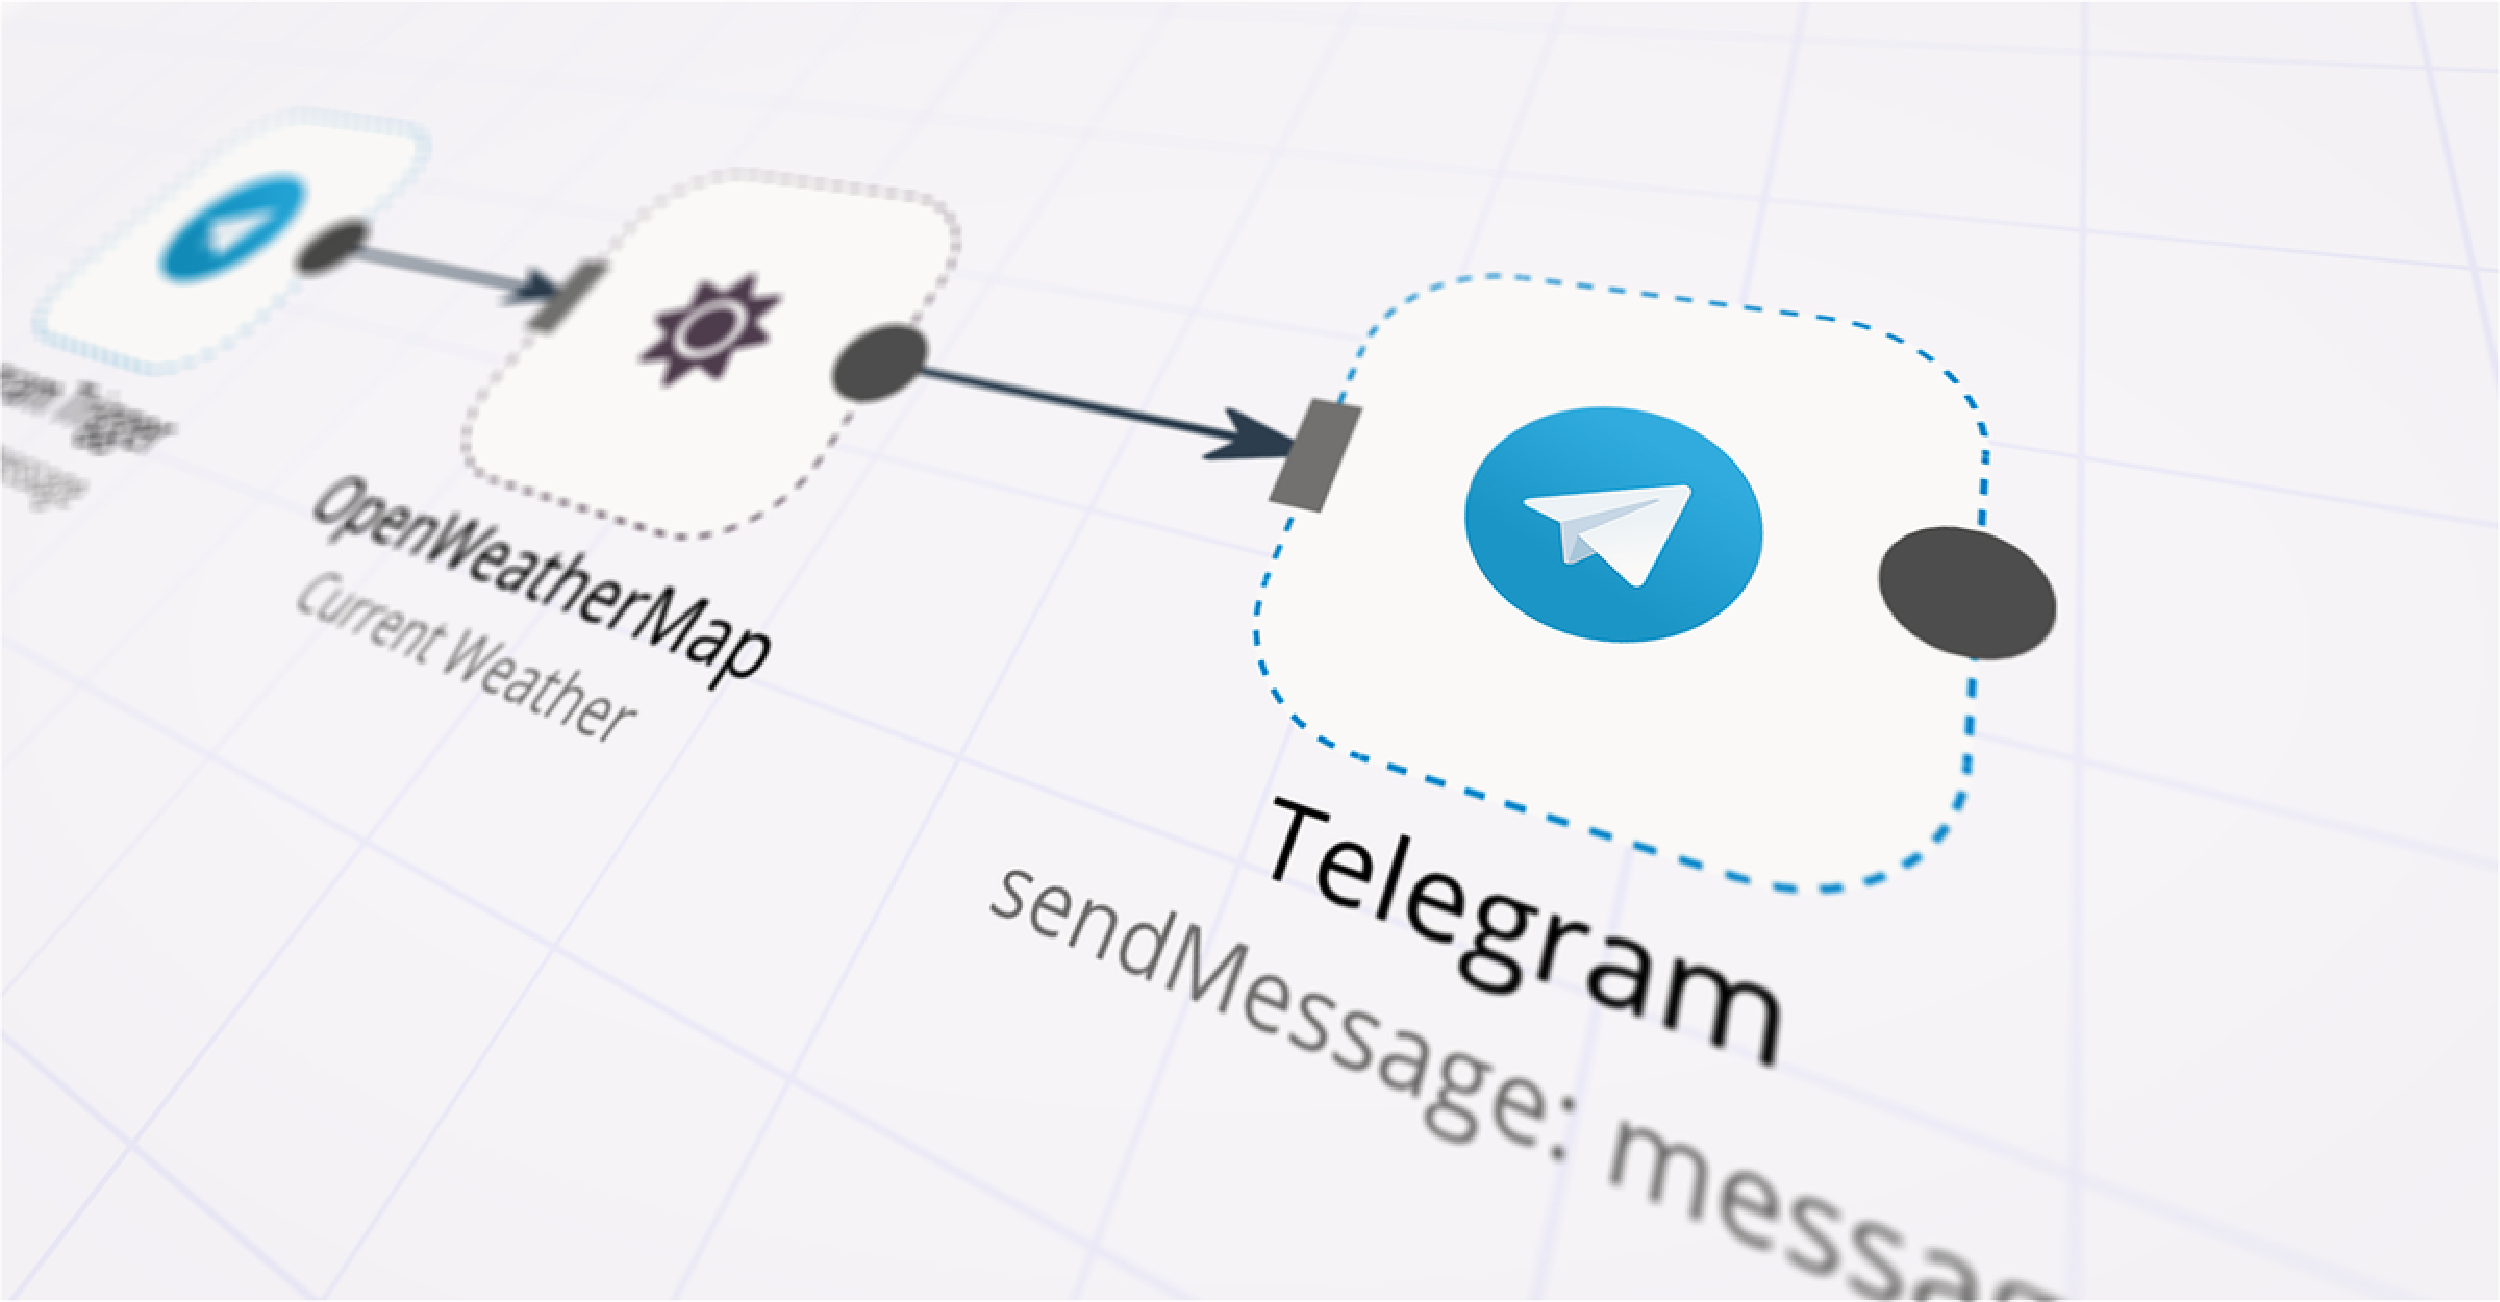
\includegraphics[width=0.8\textwidth]{Chap1-7/tele-weather.pdf}
    \caption{Workflow bot thời tiết Telegram}
\end{figure}

\textbf{Các bước thực hiện:}
\begin{enumerate}
    \item Thêm Telegram Trigger
    \item Thêm HTTP Request node:
    \begin{itemize}
        \item Method: GET
        \item URL: \verb|https://api.openweathermap.org/data/2.5/weather|
        \item Query Parameters:
        \begin{itemize}
            \item q: \verb|{{ $json.content }}| (tên thành phố từ người dùng)
            \item appid: YOUR\_API\_KEY
            \item units: metric
            \item lang: vi
        \end{itemize}
    \end{itemize}
    \item Thêm Function node để định dạng tin nhắn:
    \begin{verbatim}
    const weather = items[0].json;
    return [{
      json: {
        chatId: $node["Telegram Trigger"].json.message.chat.id,
        content: `Thời tiết tại ${weather.name}:\n` +
                 `Nhiệt độ: ${weather.main.temp}°C\n` +
                 `Độ ẩm: ${weather.main.humidity}%\n` +
                 ` Trạng thái: ${weather.weather[0].description}`
      }
    }];
    \end{verbatim}
    \item Thêm Telegram node để gửi tin nhắn lại cho người dùng
\end{enumerate}

\subsection{Xác thực API: Kết nối an toàn với dịch vụ bên ngoài}

\subsubsection{Ví dụ: Tự động đăng bài lên Facebook Page}

Để đăng bài lên Facebook, bạn cần:
\begin{enumerate}
    \item Lấy Access Token từ Facebook
    \item Sử dụng token trong API call
\end{enumerate}

Có hình
% \begin{figure}[h]
%     \centering
%     \includegraphics[width=0.8\textwidth]{images/workflow-dang-facebook}
%     \caption{Workflow đăng bài Facebook}
%     \label{fig:dang-facebook}
% \end{figure}

\textbf{Thiết lập workflow:}
\begin{enumerate}
    \item Thêm HTTP Trigger (khi có bài viết mới)
    \item Thêm HTTP Request node:
    \begin{itemize}
        \item Method: POST
        \item URL: \verb|https://graph.facebook.com/v16.0/YOUR_PAGE_ID/feed|
        \item Query Parameters:
        \begin{itemize}
            \item access\_token: YOUR\_ACCESS\_TOKEN
            \item message: \verb|{{ $json.content }}|
            \item link: \verb|{{ $json.link }}| (nếu có)
        \end{itemize}
    \end{itemize}
\end{enumerate}

\subsection{Tích hợp dịch vụ: Kết nối nhiều hệ thống}

\subsubsection{Ví dụ: Hệ thống CRM đơn giản}

Khi có khách hàng mới từ website:
\begin{enumerate}
    \item Lưu thông tin vào Google Sheets
    \item Tạo task theo dõi trong Trello
    \item Gửi email thông báo cho nhân viên
\end{enumerate}

Có hình
% \begin{figure}[h]
%     \centering
%     \includegraphics[width=0.8\textwidth]{images/workflow-crm-don-gian}
%     \caption{Workflow CRM đơn giản}
%     \label{fig:crm-don-gian}
% \end{figure}

\textbf{Các bước thực hiện:}
\begin{enumerate}
    \item Thêm Webhook node (nhận thông tin từ form)
    \item Thêm Google Sheets node:
    \begin{itemize}
        \item Operation: Append
        \item Spreadsheet: Danh sách khách hàng
        \item Range: Sheet1!A:E
    \end{itemize}
    \item Thêm Trello node:
    \begin{itemize}
        \item Operation: Create Card
        \item List: Khách hàng mới
        \item Title: \verb|Liên hệ {{ $json.hoTen }}|
        \item Description: \verb|{{ $json.email }} - {{ $json.soDienThoai }}|
    \end{itemize}
    \item Thêm Send Email node để thông báo cho nhân viên
\end{enumerate}

\subsection{Xử lý lỗi API: Đảm bảo workflow hoạt động ổn định}

\subsubsection{Ví dụ: Backup dữ liệu từ hệ thống cũ sang mới}

Khi chuyển dữ liệu, cần xử lý các trường hợp lỗi:

Có hình
% \begin{figure}[h]
%     \centering
%     \includegraphics[width=0.8\textwidth]{images/workflow-xu-ly-loi-api}
%     \caption{Workflow xử lý lỗi API}
% \end{figure}

\textbf{Thiết lập workflow:}
\begin{enumerate}
    \item Thêm Trigger (bắt đầu chuyển dữ liệu)
    \item Thêm HTTP Request node để lấy dữ liệu từ hệ thống cũ
    \item Thêm IF node để kiểm tra kết quả:
    \begin{itemize}
        \item Condition: \verb|{{ $json.statusCode }}| Equals \verb|200|
    \end{itemize}
    \item Nếu thành công:
    \begin{itemize}
        \item Thêm HTTP Request để gửi dữ liệu lên hệ thống mới
    \end{itemize}
    \item Nếu thất bại:
    \begin{itemize}
        \item Thêm Send Email node để thông báo lỗi
        \item Lưu lỗi vào log file
    \end{itemize}
\end{enumerate}

\newpage
\section{Bài tập thực hành}
\begin{enumerate}
    \item Tạo workflow gửi email chào mừng khách hàng mới với biến \verb|welcomeMessage| và \verb|companyName|.
    \item Thiết lập workflow tính giá sau giảm giá 15\% với Expressions và định dạng giá tiền.
    \item Thiết kế workflow lưu số lượt truy cập website bằng Data Storage.
    \item Xây dựng workflow cache kết quả giá vàng từ API trong 30 phút bằng Cache node.
    \item Tạo workflow lưu đơn hàng vào database và gửi email thông báo cho admin.
    \item Tạo bot Telegram trả lời thông tin thời tiết dựa trên tên thành phố người dùng gửi.
    \item Thiết lập workflow tự động đăng bài lên Facebook Page sử dụng API và Access Token.
    \item Xây dựng workflow nhận khách hàng mới từ website, lưu vào Google Sheets và tạo thẻ Trello.
    \item Tạo workflow backup dữ liệu giữa hai hệ thống, xử lý lỗi API và gửi email khi thất bại.
\end{enumerate}